Dieses Kapitel beschäftigt sich mit der Analyse und der Bewertung von den eingeführten Verfahren aus den Kapiteln \ref{chp:sichtpruefungDurchLichtstreuung} und \ref{chp:deflektometrischeRegistrierung} zur Auswertung von Oberflächeninformationen spiegelnder Prüfobjekte.
Im Anschluss an die Beschreibung der Ergebnisse der einzelnen Verfahren soll eine Diskussion und ein Vergleich der Ergebnisse erfolgen.

\p
Die angegebenen Ergebnisse in diesem Abschnitt wurden auf einem Computer mit Intel(R) Core(TM) i5-7400 CPU @3.00GHz, 4 Kerne, 8GB Arbeitsspeicher, Intel(R) HD Graphics 630 und Microsoft Windows 10 Pro (10.0, Build 19044) erreicht.
Die Implementierung der Verfahren erfolgte als Plug-in für die Software NeuroCheck (Version 6.2) in der Programmiersprache C\#.
NeuroCheck ist ein Bildverarbeitungssystem zur Erstellung von Prüfprogrammen für die optische Qualitätssicherung.
Nach einem Baukastenprinzip lassen sich Lösungen für individuelle Problemstellungen in den Bereichen der industriellen Bildverarbeitung entwickeln.
Über das Plug-in Interface von NeuroCheck können selbst entworfene Funktionen in die Software integriert und mit einer großen Auswahl von angebotenen Methoden weiterverarbeitet werden.

% Abbildung: Fotos der verwendeten Aufbauten
{
	\begin{figure}[H]
		\centering
		\begin{tikzpicture}[every node/.style={inner sep=0,outer sep=0}]

	\node [anchor=north east] (imgAufbauDurchlicht) at (-0.03\textwidth,0) {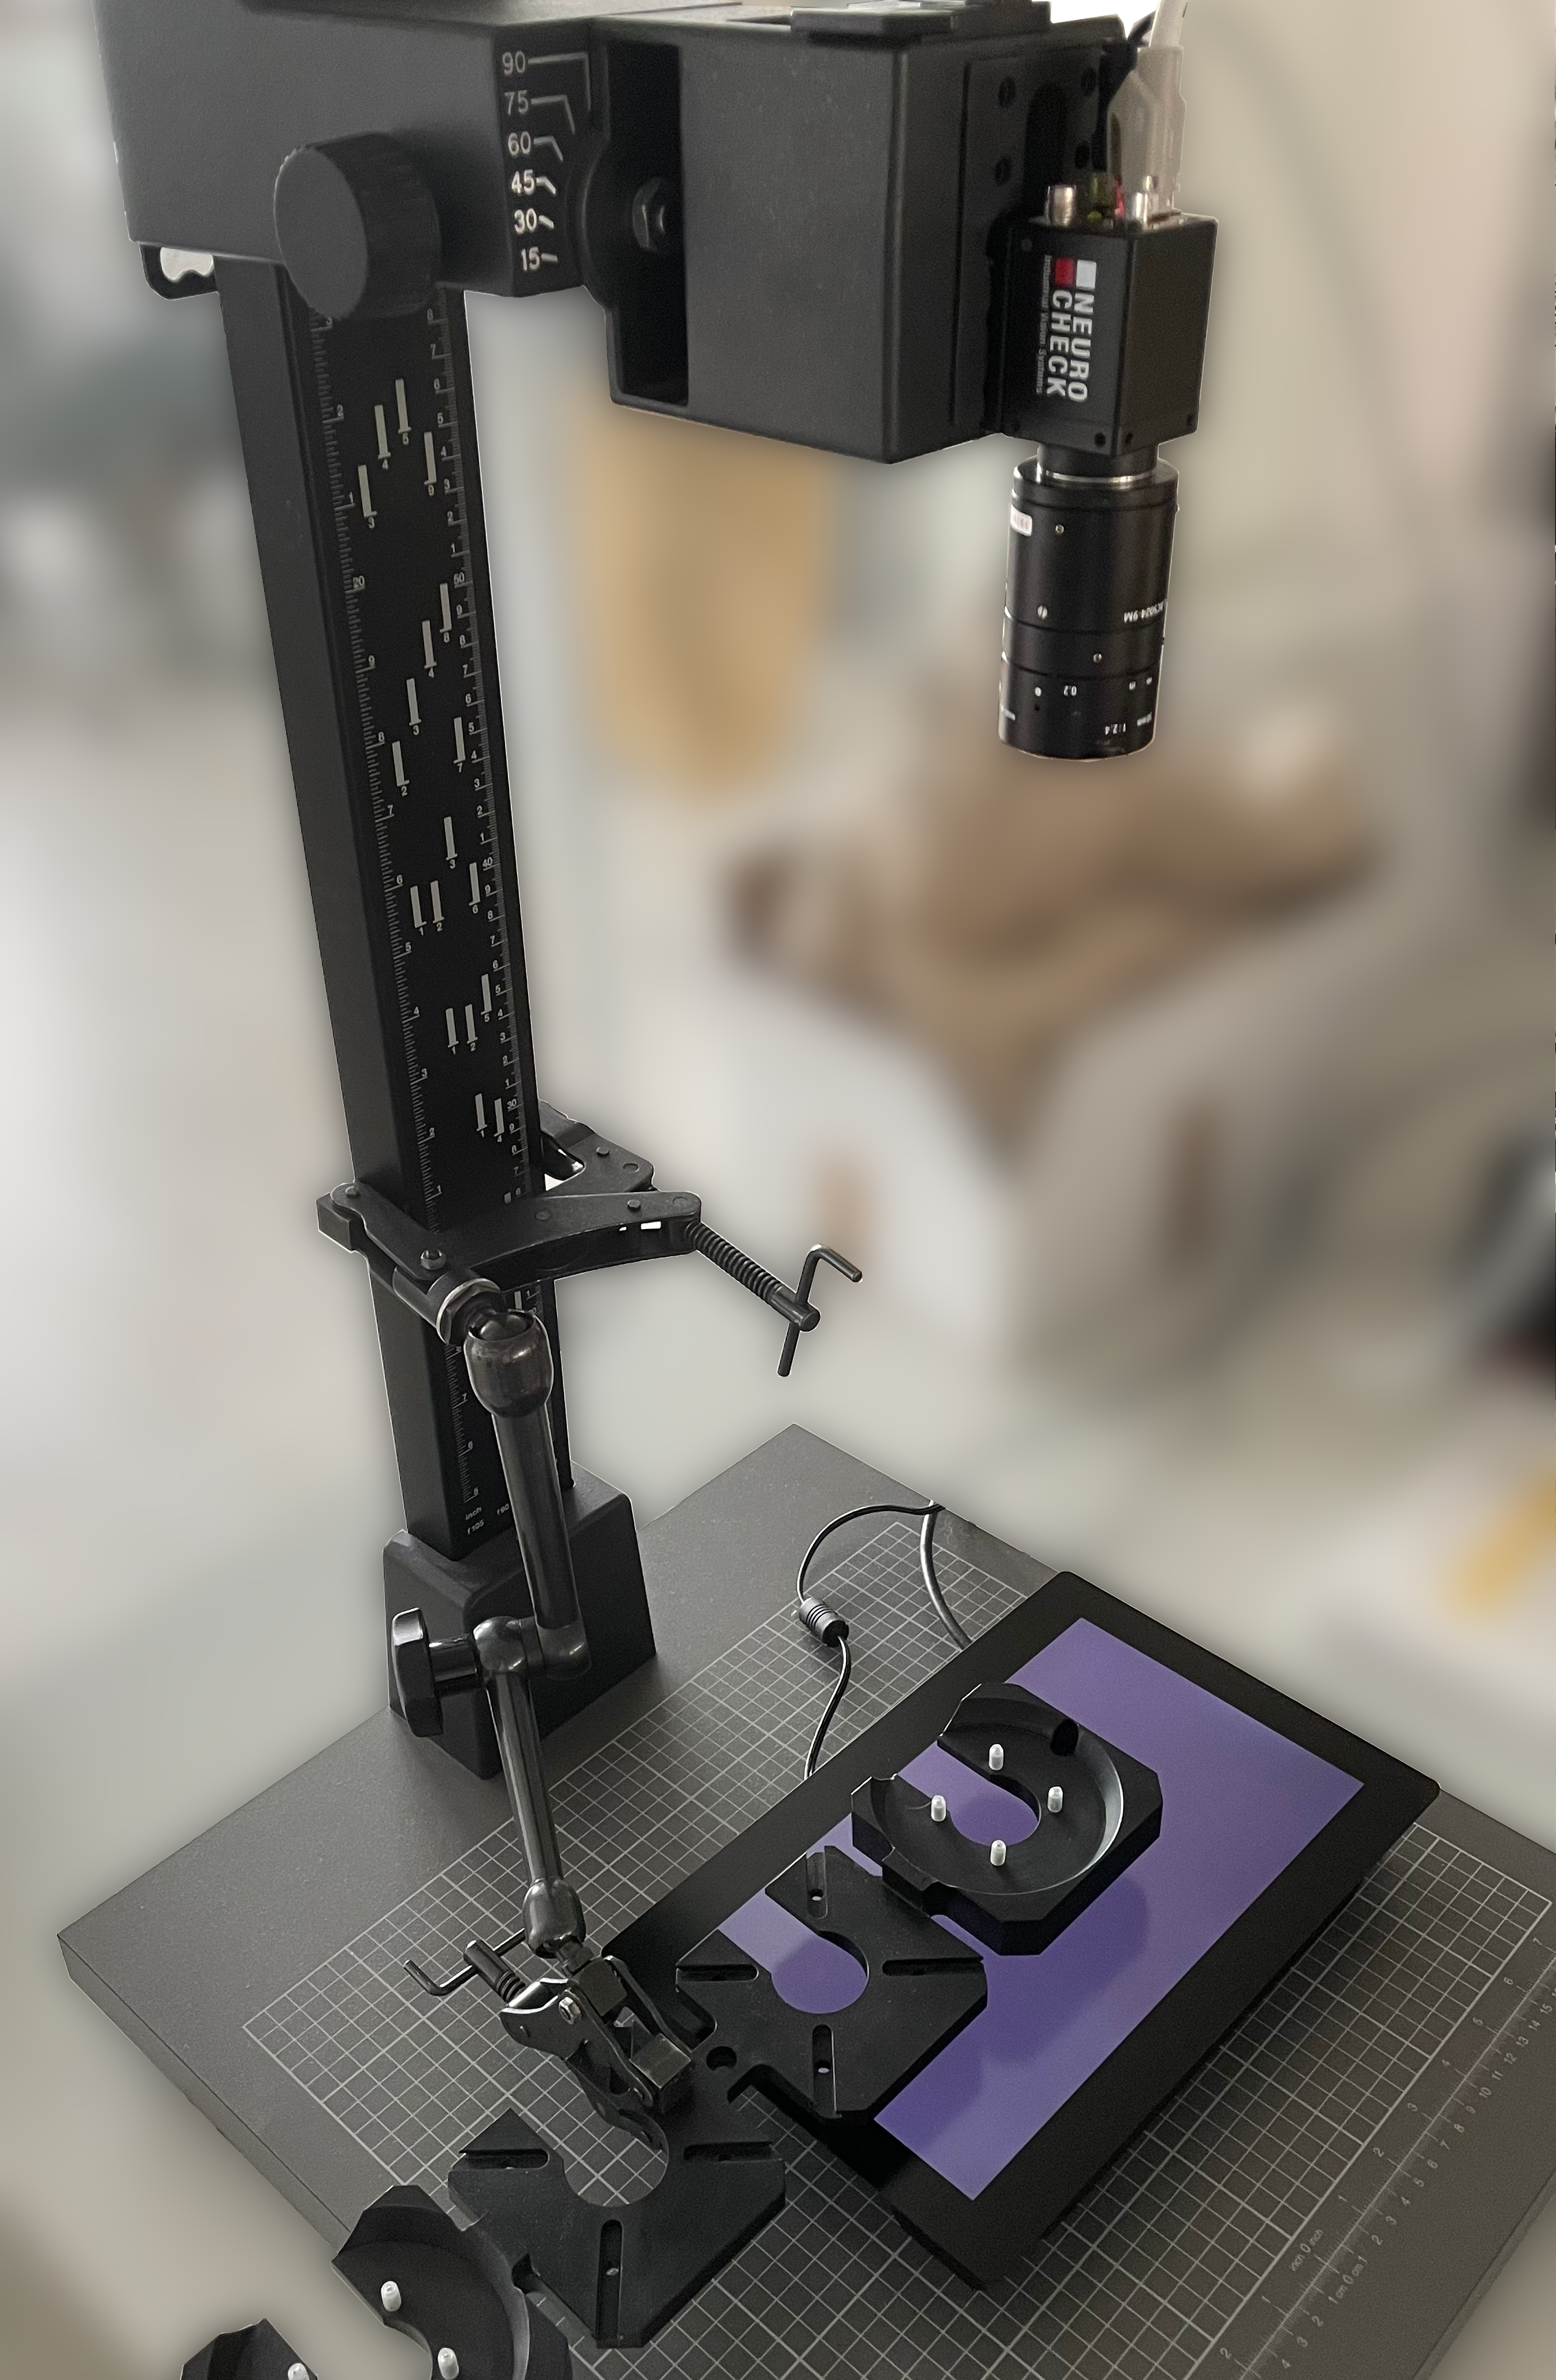
\includegraphics[width=.3\textwidth]{05_ergebnisse/figures/aufbauFotoDurchlicht}};
	\node [below=0.2cm of imgAufbauDurchlicht] {Durchlichtauswertung};
	\node [anchor=north west] (imgAufbauReflexion) at (0.03\textwidth,0) {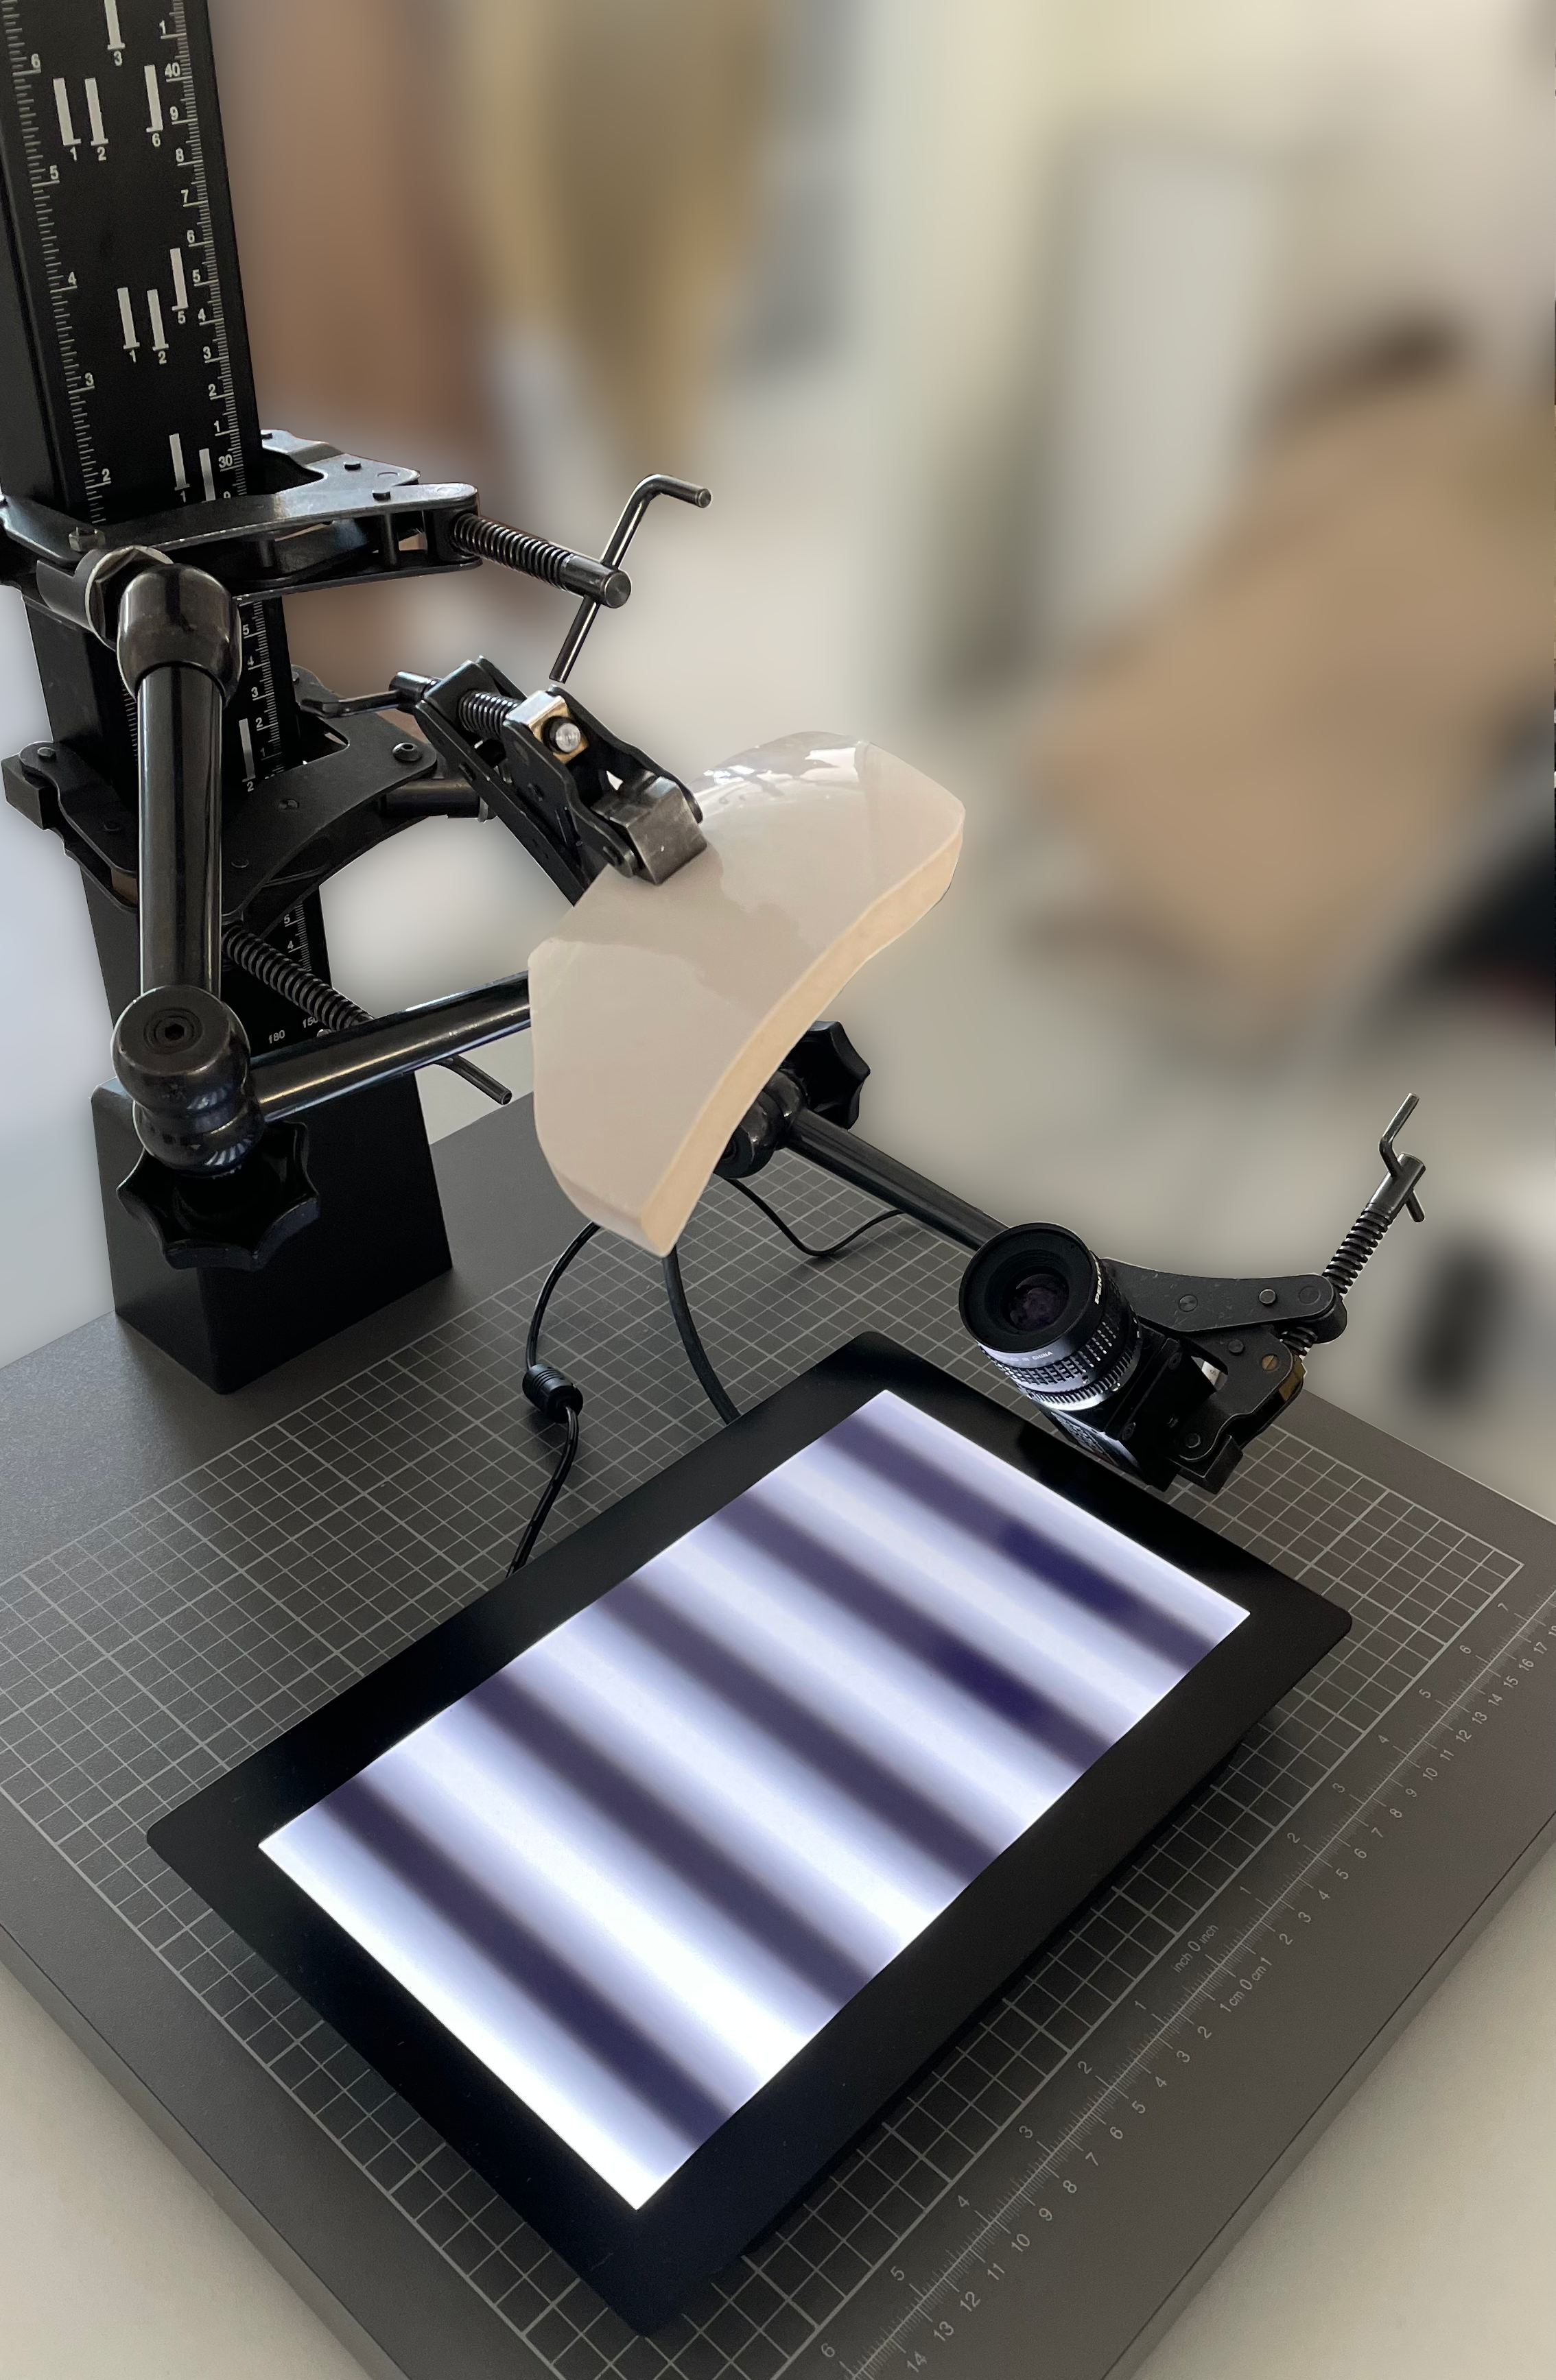
\includegraphics[width=.3\textwidth]{05_ergebnisse/figures/aufbauFotoReflexion}};
	\node [below=0.2cm of imgAufbauReflexion] {Spiegelbildauswertung};
	
\end{tikzpicture}
\caption[Fotos der verwendeten Aufbauten für die Verfahren]{Fotos der verwendeten Aufbauten für die Verfahren}
		\label{tikz:abbAufbauFotos}
	\end{figure}
}

\noindent
Abbildung \ref{tikz:abbAufbauFotos} zeigt die verwendeten Aufbauten zur Erzeugung von Bildern für die Verfahren.
Die Durchlichtauswertung eignet sich nur für transparente Prüfobjekte, während die Spiegelbildauswertung allgemein auf spiegelnde Prüfobjekte, also auch auf transparente Prüfobjekte, anwendbar ist.
Die verwendeten Kamerabilder haben eine Auflösung von 500 x 370 Pixeln und umfassen nur die Helligkeitsstufen. 
Das heißt, es werden nur Graubilder verarbeitet.
Bei den folgenden Aufnahmen gilt zu berücksichtigen, dass ein spezieller Polarisationsfilter fest auf der verwendeten Kamera angebracht ist.
In den Aufnahmen ergibt sich dadurch stets eine Struktur aus Streifen mit diagonaler Ausbreitungsrichtung von oben links nach unten rechts.
Die Objektive wurden an die jeweilige Szene angepasst, um geeignete Bilder aufnehmen zu können.
Zur Verbesserung der Ergebnisse werden die verwendeten Aufbauten noch durch geeignete Abschirmungen vor Fremdlicht geschützt.

%Sichtprüfung durch Lichtstreuung
{
	\FloatBarrier
    \section{Sichtprüfung durch Lichtstreuung}
    \label{sec:ergebnisseSichtpruefungDurchLichtstreuung}
    Das Verfahren \glqq Sichtprüfung durch Lichtstreuung\grqq ~wurde in Kapitel \ref{chp:sichtpruefungDurchLichtstreuung} eingeführt und lässt kleine Defekte auf spiegelnden Oberflächen sichtbar werden.

\begin{table}[H]
	\centering
	\label{tab:paramSichtpruefung}
	\begin{tabular}{lll}
		\hline 
		\textbf{Beschreibung} & \textbf{Name} & \textbf{Wert} \\ 
		\hline 
		Tastgrad (beeinflusst die Streifenbreiten) & $D$ & $\tfrac{2}{5}$ \\ 
		Amplitude (beeinflusst die Helligkeit) & $A_m$ & 127.5 \\ 
		Kontrast & $C_m$ & 1.0 \\ 
		Anzahl Phasenverschiebungen & $N_{shift}$ & 16 \\ 
		Bildschirmbreite (in Pixel) & \acrshort{lwidth} & 1920 \\
		Bildschirmhöhe (in Pixel) & \acrshort{lheight} & 1080 \\ 
		\hline 
	\end{tabular}
	\caption{Parameter des Verfahrens}
\end{table}
}

%Deflektometrische Registrierung
{
	\FloatBarrier
    \section{Deflektometrische Registrierung}
    \label{sec:ergebnisseDeflektometrischeRegistrierung}
    Das Verfahren zur Bestimmung der \glqq deflektometrischen Registrierung\grqq ~wurde in Kapitel \ref{chp:deflektometrischeRegistrierung} eingeführt und bestimmt eine Zuordnung zwischen Bildschirm- und Kamerapunkten.
Nach Abschnitt \ref{sec:auswertungDeflektometrischeRegistrierung} lässt sich diese Zuordnung auswerten und als Bilder darstellen.

\begin{table}[H]
	\centering
	\label{tab:paramDeflektometrischRegistrierung}
	\begin{tabular}{lll}
	\hline 
	\textbf{Beschreibung} & \textbf{Name} & \textbf{Wert} \\ 
	\hline 
	Amplitude (beeinflusst die Helligkeit) & $A_m$ & 127.5 \\
	Kontrast & $C_m$ & 1.0 \\
	Anzahl Perioden des ersten Muster & $N_p^1$ & 3 \\ 
	Anzahl Perioden des zweiten Muster & $N_p^2$ & 5 \\ 
	Anzahl Perioden des dritten Muster & $N_p^3$ & 7 \\  
	Anzahl Phasenverschiebungen jedes Musters & $N_{shift}$ & 16 \\ 
	Bildschirmbreite (in Pixel) & \acrshort{lwidth} & 1920 \\
	Bildschirmhöhe (in Pixel) & \acrshort{lheight} & 1080 \\
	\hline 
	\end{tabular} 
	\caption{Parameter des Verfahrens}
\end{table}
}

%Diskussion
{
	\FloatBarrier
    \section{Diskussion}
    \label{sec:diskussion}
    Im Folgenden sollen die beschriebenen Ergebnisse aus den vorherigen Abschnitten \ref{sec:ergebnisseSichtpruefungDurchLichtstreuung} und \ref{sec:ergebnisseDeflektometrischeRegistrierung} aufgegriffen und bewertet werden.
Das Ziel ist es abhängig vom Anwendungsfall ein passendes Verfahren vorzuschlagen und die Schwächen und Stärken der Verfahren anzusprechen.

\p
Für das Verfahren \glqq Sichtprüfung durch Lichtstreuung\grqq ~fällt im Abschnitt \ref{sec:ergebnisseSichtpruefungDurchLichtstreuung} auf, dass es sich besonders gut für die Durchlichtauswertung von transparenten Prüfobjekten eignet.
Es ist möglich bereits sehr kleine Defekte, wie z. B. sehr leichte Kratzer oder Laser-Gravuren auf den Objektoberflächen zu erkennen (siehe Abbildung \ref{tikz:abbErkennbareKleineDefekteLichtstreuung}).

% Abbildung: Erkennbare kleine Defekte
{
	\begin{figure}[H]
		\centering
		\begin{tikzpicture}[every node/.style={inner sep=0,outer sep=0}]

	\node [anchor=north east] (img1) at (-0.03\textwidth,0) {\includegraphics[width=.4\textwidth]{05_ergebnisse/ergDiskussion/figures/lasergravur}};
	\node [below=0.2cm of img1, align=center] {Ausschnitt von Brillenglas 1 \\ aus Abbildung \ref{tikz:abbNachbearbeitung}};
	\node [anchor=north west] (img2) at (0.03\textwidth,0) {\includegraphics[width=.4\textwidth]{05_ergebnisse/ergDiskussion/figures/polierfehler}};
	\node [below=0.2cm of img2, align=center] {Ausschnitt von Brillenglas 2 \\ aus Abbildung \ref{tikz:abbNachbearbeitung}};
	
\end{tikzpicture}
\caption[Erkennbare kleine Defekte oder Laser-Gravur]{Erkennbare kleine Defekte oder Laser-Gravuren durch Durchlichtauswertung mit Verfahren \glqq Sichtprüfung durch Lichtstreuung\grqq ~(siehe Kapitel \ref{chp:sichtpruefungDurchLichtstreuung}). Linkes Teilbild: Erkennbare Lasergravur, Rechtes Teilbild: Leichte Kratzer durch Fehler bei der Polierung}
		\label{tikz:abbErkennbareKleineDefekteLichtstreuung}
	\end{figure}
}

\noindent
Außerdem ist es möglich für transparente Objekte durch die Durchlichtauswertung auch Defekte im Objekt, wie z. B. Lufteinschlüsse in Gläsern festzustellen.
Dies konnte allerdings nicht nachgeprüft werden, da solche Defekte in den zur Verfügung stehenden Prüfobjekten nicht vorhanden waren.

\p
Für nicht-transparente kann das Verfahren \glqq Sichtprüfung durch Lichtstreuung\grqq ~ebenfalls verwertbare Bilder erzeugen um Defekte zu detektieren, allerdings gibt es hierbei schon erste Probleme.
Eine große Schwäche des Verfahrens ist die Abhängigkeit von Oberflächenbeschriftungen oder -aufdrucken.
Da stets Grauwerte der Kamerabilder verknüpft werden beeinflussen unterschiedliche Farben auf der Oberfläche das Ergebnis (siehe Abbildung \ref{img:delleBeschriftung}).

% Abbildung: Beschriftung Delle
{
	\begin{figure}[H]
		\centering
		\includegraphics[width=0.4\textwidth]{05_ergebnisse/ergDiskussion/figures/delleBeschriftung}
		\caption[Sichtbare Beschriftung nach Anwendung des Verfahrens aus Kapitel \ref{chp:sichtpruefungDurchLichtstreuung}]{Sichtbare Beschriftung \glqq Delle\grqq ~nach Anwendung des Verfahren \glqq Sichtprüfung durch Lichtstreuung\grqq.}
		\label{img:delleBeschriftung}
	\end{figure}
}
}